\documentclass[12pt,letterpaper]{article}
\usepackage[utf8]{inputenc}
\usepackage[spanish]{babel}
\usepackage{graphicx}
\usepackage[left=2cm,right=2cm,top=2cm,bottom=2cm]{geometry}
\usepackage{graphicx} % figuras
% \usepackage{subfigure} % subfiguras
\usepackage{float} % para usar [H]
\usepackage{amsmath}
%\usepackage{txfonts}
\usepackage{stackrel} 
\usepackage{multirow}
\usepackage{enumerate} % enumerados
\renewcommand{\labelitemi}{$-$}
\renewcommand{\labelitemii}{$\cdot$}
% \author{}
% \title{Caratula}
\begin{document}

% Fancy Header and Footer
% \usepackage{fancyhdr}
% \pagestyle{fancy}
% \cfoot{}
% \rfoot{\thepage}
%

% \usepackage[hidelinks]{hyperref} % CREA HYPERVINCULOS EN INDICE

% \author{}
\title{Caratula}

\begin{titlepage}
\begin{center}
\large{UNIVERSIDAD PRIVADA DE TACNA}\\
\vspace*{-0.025in}
\begin{figure}[htb]
\begin{center}

\includegraphics[width=8cm]{./Imagenes/logo}
\end{center}
\end{figure}
\vspace*{0.15in}
INGENIERIA DE SISTEMAS  \\

\vspace*{0.5in}
\begin{large}
TITULO:\\
\end{large}

\vspace*{0.1in}
\begin{Large}
\textbf{INFORME DE LABORATORIO No 02} \\
\end{Large}

\vspace*{0.3in}
\begin{Large}
\textbf{CURSO:} \\
\end{Large}

\vspace*{0.1in}
\begin{large}
INTELIGENCIA DE NEGOCIOS \\
\end{large}

\vspace*{0.3in}
\begin{Large}
\textbf{DOCENTE(ING):} \\
\end{Large}

\vspace*{0.1in}
\begin{large}
 Patrick Cuadros Quiroga\\
\end{large}

\vspace*{0.2in}
\vspace*{0.1in}
\begin{large}
Alumno: \\
\begin{flushleft}
Zegarra Reyes Roberto CArlos		\hfill	(2010036175) \\

\end{flushleft}
\end{large}
\end{center}

\end{titlepage}


\tableofcontents % INDICE
\thispagestyle{empty} % INDICE SIN NUMERO
\newpage
\setcounter{page}{1} % REINICIAR CONTADOR DE PAGINAS DESPUES DEL INDICE

\section{Ejercicio 1: Crear relaciones - Tarea 1: Relaciones automáticas} 



\begin{enumerate}[1.]
	\item  Ingresar a Power BI Desktop. En la Ventana de Power BI Desktop, click en Obtener Datos (Get Data). En el cuadro de dialogo Obtener Datos (Get Data), asegurarse que Excel esta seleccionado y hacer click en Conectar (Connect).
	En el cuadro de dialogo Abrir (Open), buscar el archivo Adventure Works Sales Data.xlsx, y luego hacer
click en Abrir (Open).	 En el cuadro de dialogo Explorador (Navigator), seleccionar las hojas DimCurrency, DimCustomer,
DimDate, DimProduct, DimPromotion, DimSalesTerritory, y FactInternetSales.
	
	

	\begin{center}
	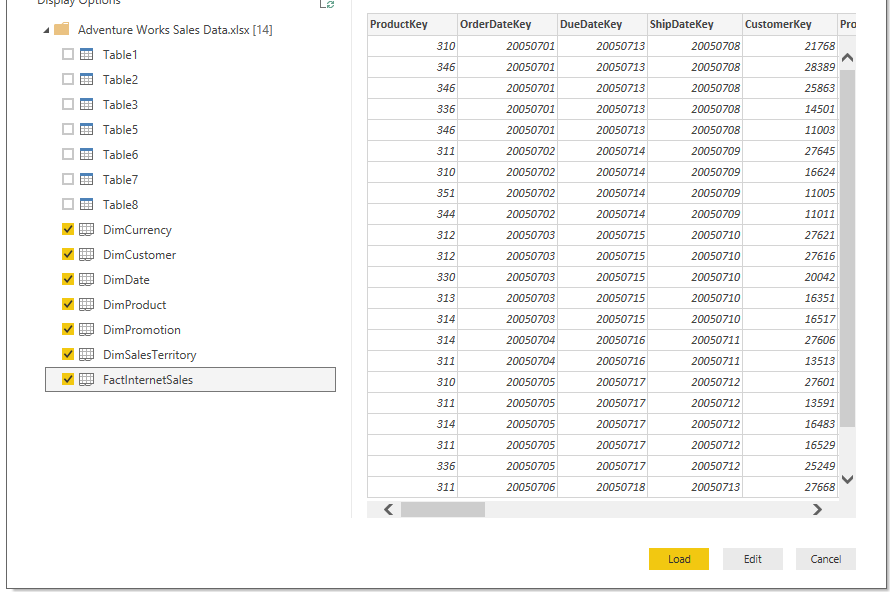
\includegraphics[width=11cm]{./Imagenes/11} 
	\end{center}


	\item   En el panel de vistas a mano derecho, hacer click en Relaciones (Relationships).
 En el menú principal, hacer click en Administrar relaciones (Manage Relationships).

	\begin{center}
	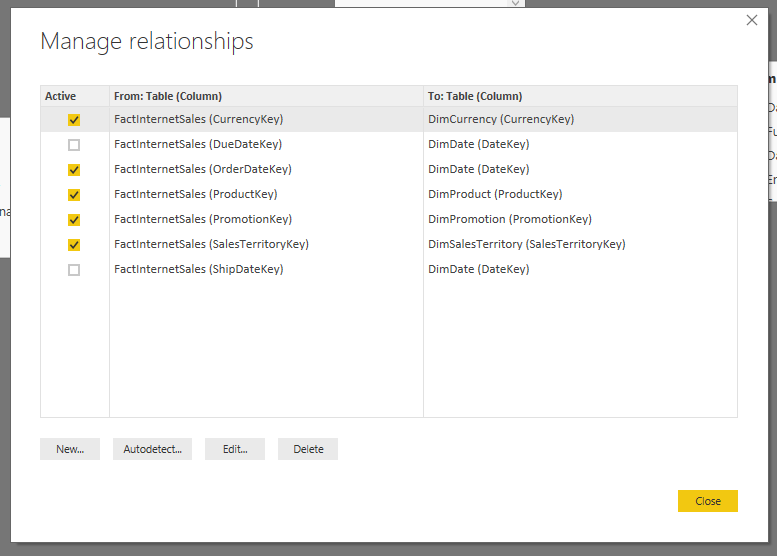
\includegraphics[width=11cm]{./Imagenes/12} 
	\end{center}



\item En el menú principal, hacer click en Administrar relaciones (Manage Relationships). En el cuadro de Administrar relaciones (Manage Relationships), hacer click en Nueva (New). En la lista de tablas superior, hacer click en FactInternetSales. Luego hacer click en la columna CustomerKey en la vista de datos previa. En la lista de tablas superior, hacer click en DimCustomer, y hacer click CustomerKey en la vista de datos previa. En la lista de Cardinalidad (Cardinality), hacer click en Muchos a Uno (Many to One (*:1)), y luego hacer click en Aceptar (OK).
	\begin{center}
	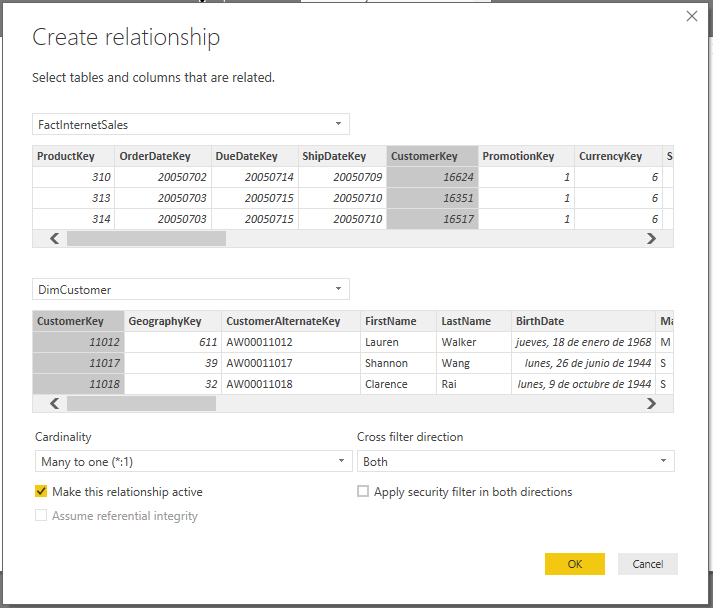
\includegraphics[width=12cm]{./Imagenes/13} 
	\end{center}

\item Cargar el archive como Ventas Adventure Works.pbix.
	\begin{center}
	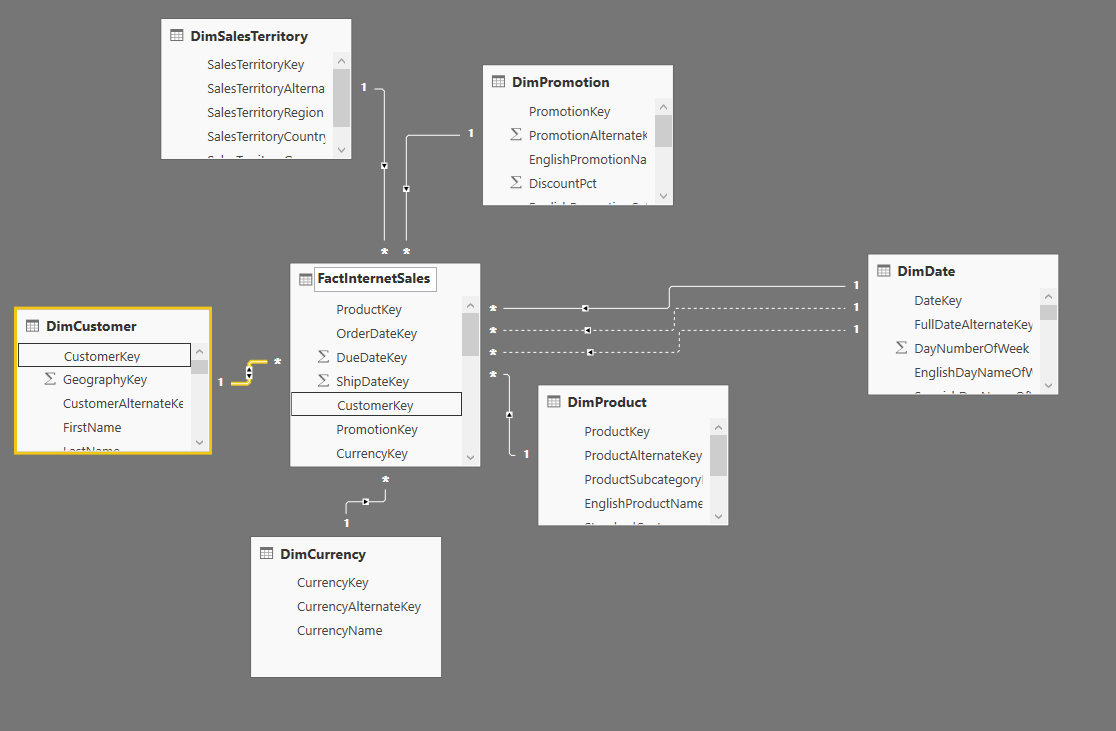
\includegraphics[width=12cm]{./Imagenes/14} 
	\end{center}

\end{enumerate}





\section{Ejercicio 1: Crear relaciones - Tarea 2: Relaciones manuales} 

\begin{enumerate}[1.]
	\item En la Ventana de Power BI Desktop, click en Obtener Datos (Get Data) y luego en Excel. Abrir el archivo Adventure Works Product Categories.xlsx. En el cuadro de dialogo Explorador (Navigator), seleccionar las hojas DimProductCategory, and
DimProductSubcategory, y luego hacer click en Cargar (Load).
	
	\begin{center}
	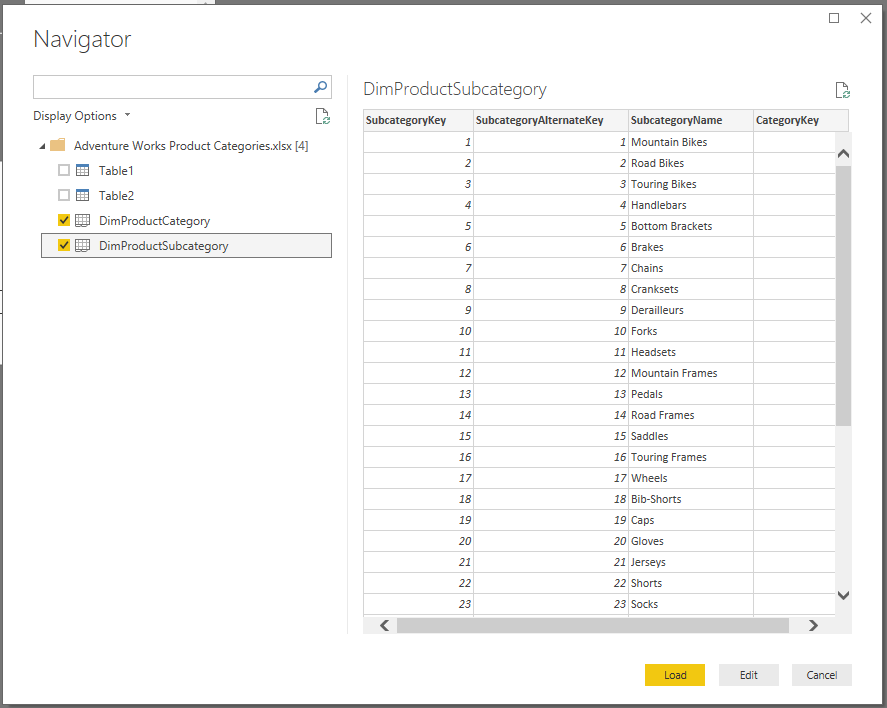
\includegraphics[width=11cm]{./Imagenes/21} 
	\end{center}

	\item En el panel de Relaciones, revisar la relación que Power BI ha creado entre las dos tablas.
 Hacer click en la línea de la relación entre DimProductCategory, y DimProductSubcategory, y seleccionar
Eliminar (Delete). En el cuadro de dialogo Eliminar relación (Delete Relationship), hacer click en Borrar (Delete).

	

	\begin{center}
	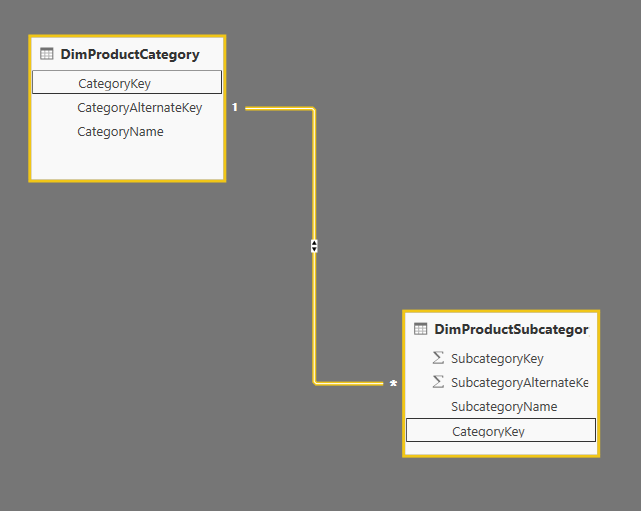
\includegraphics[width=9cm]{./Imagenes/22} 
	\end{center}

	\item Arrastrar la columna CategoryKey en la tabla DimProductSubcategory a la columna Category en la tabla
DimProductCategory, para crear una relación Muchos a uno (Many to One (*:1)), y una dirección de filtro
cruzado (Cross filter direction) en ambos

	
	\begin{center}
	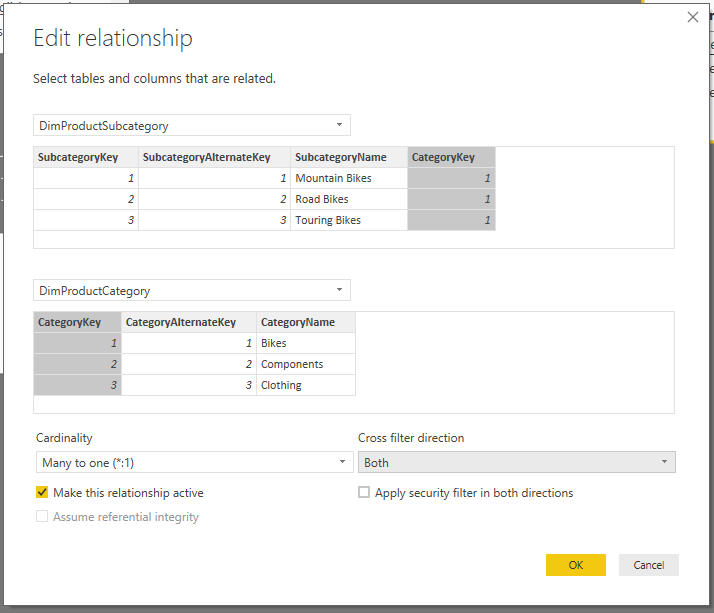
\includegraphics[width=11cm]{./Imagenes/23} 
	\end{center}


	\item En la tabla DimProduct, arrastrar la columna ProductSubcategoryKey a la columna SubcategoryKey en la tabla DimProductSubcategory, para crear una relación de Muchos a Uno (Many to One (*:1)), y una dirección de filtro cruzado (Cross filter direction) en ambos.
	
	\begin{center}
	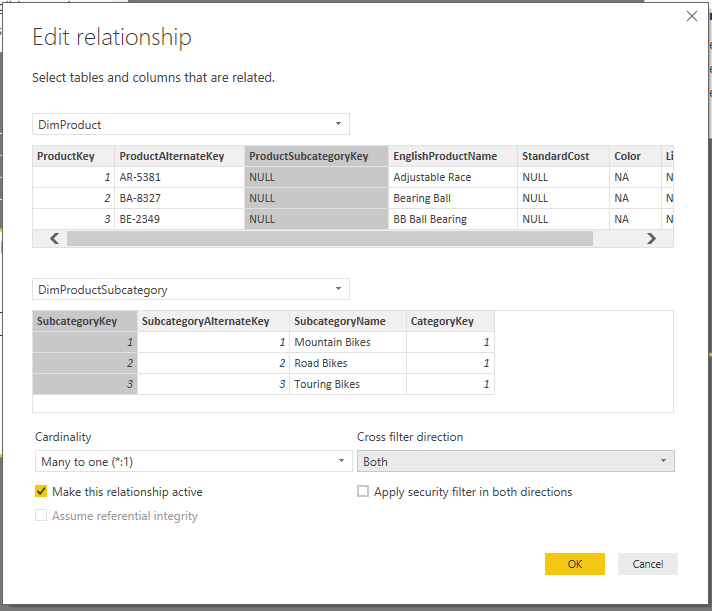
\includegraphics[width=11cm]{./Imagenes/24} 
	\end{center}

	\item Hacer click en Guardar
	
	\begin{center}
	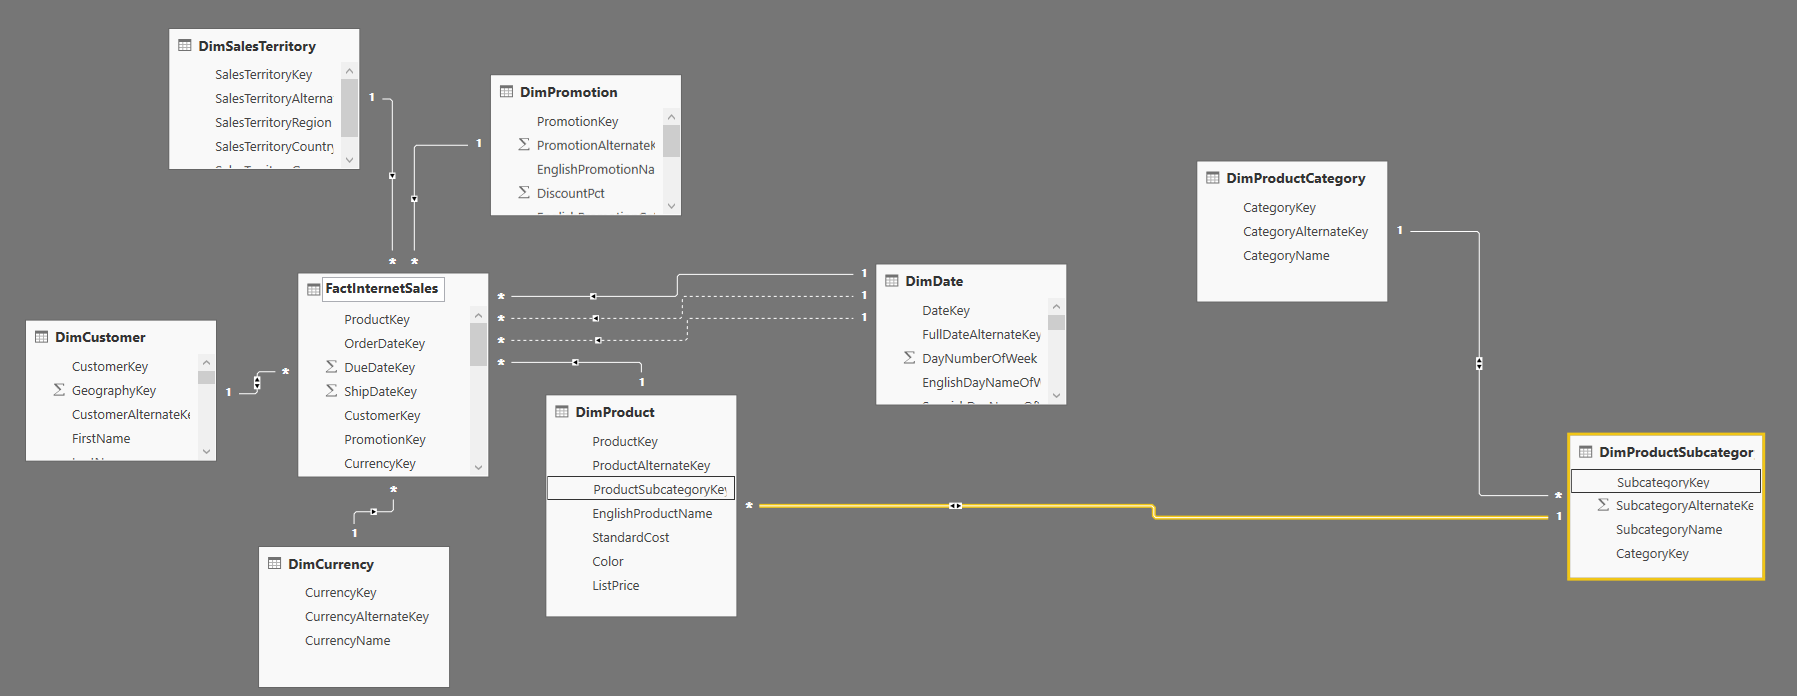
\includegraphics[width=18cm]{./Imagenes/25} 
	\end{center}

\end{enumerate}



\section{Ejercicio 2: Cálculos} 
		
\begin{enumerate}[1.]
	\item  En Power BI Desktop, haga clic en Datos en el panel de vistas en el lado izquierdo. En el panel Campos, haga clic en DimCustomer.  En la cinta Modelado, en el grupo Cálculos, haga clic en Nueva columna. En la barra de fórmulas, resalte Columna = y escriba:
	\\	
	\\
	\\IncomeStatus = IF (DimCustomer[YearlyIncome] < 25000, "Lower Income", \\
	  IF (AND(DimCustomer[YearlyIncome] >= 25000, DimCustomer[YearlyIncome] < 60000),\\
	  "Middle Income", \\
	   IF (AND(DimCustomer[YearlyIncome] >= 60000, DimCustomer[YearlyIncome] < 100000), \\
	"Higher Income", \\
	IF (DimCustomer[YearlyIncome] >= 100000, "Very High Income", "Other")))) \\

	\begin{center}
	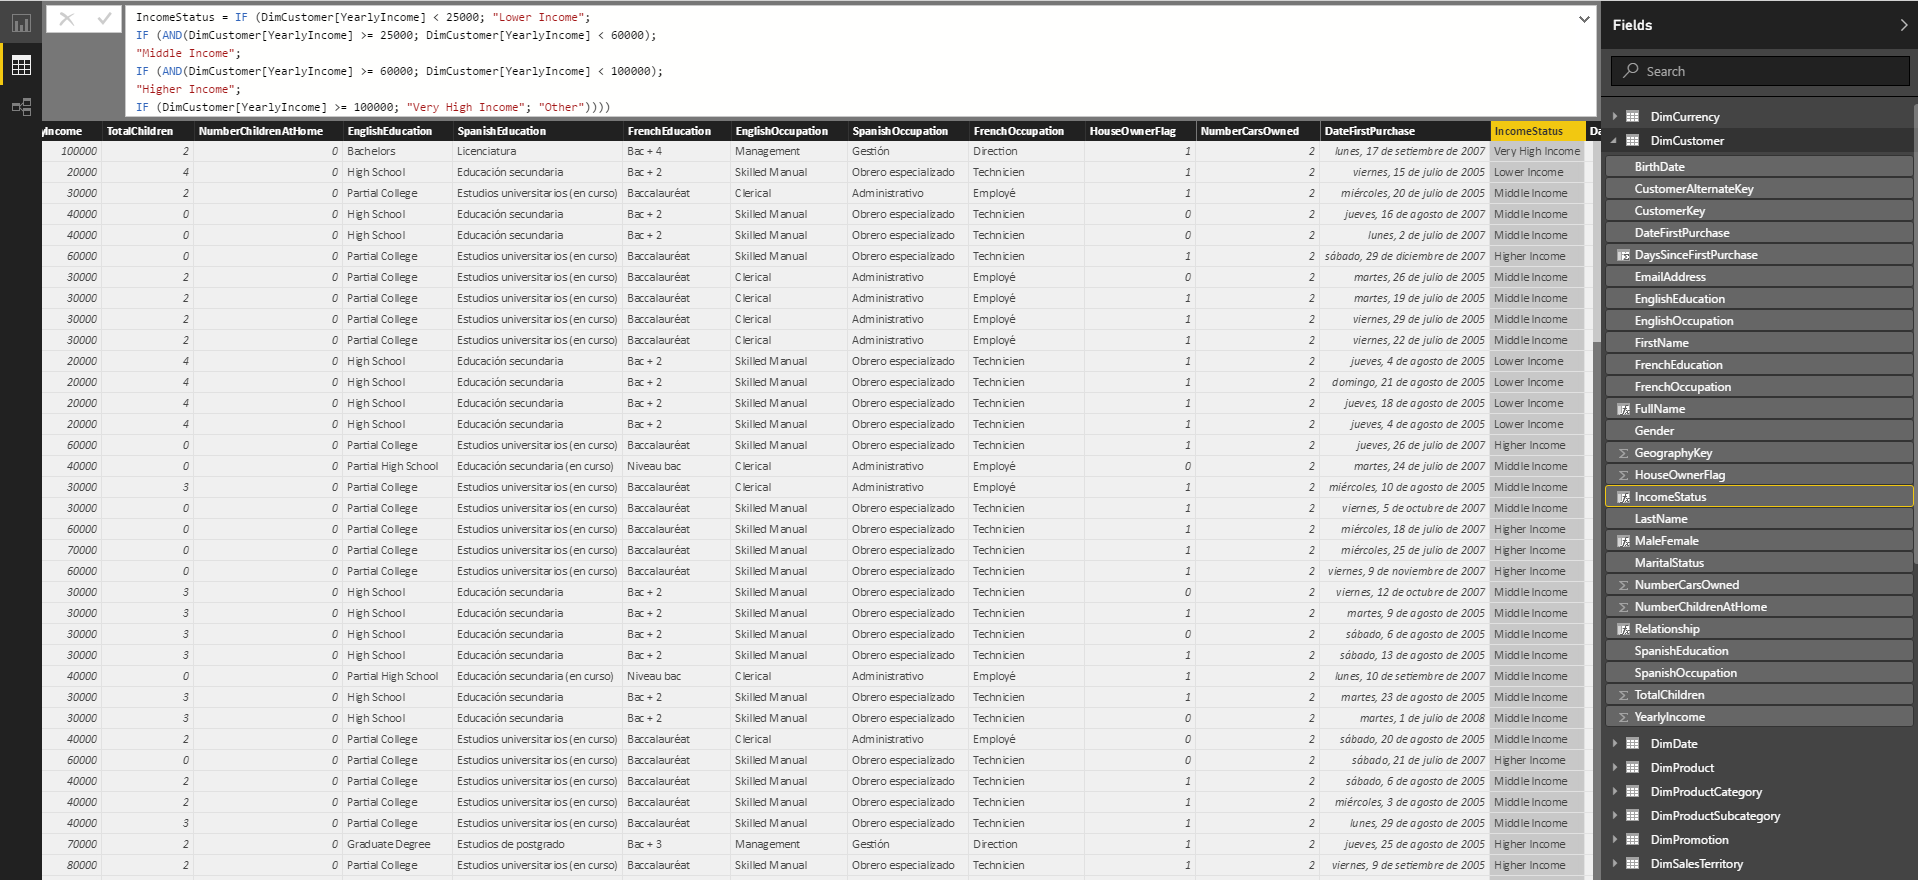
\includegraphics[width=17cm]{./Imagenes/31} 
	\end{center}

	\item  En Power BI Desktop, haga clic en Datos en el panel de vistas en el lado izquierdo. En el panel Campos, haga clic en DimCustomer.  En la cinta Modelado, en el grupo Cálculos, haga clic en Nueva columna. En la barra de fórmulas, resalte Columna = y escriba:
	\\
	\\
	\\DaysSinceFirstPurchase = DATEDIFF(DimCustomer[DateFirstPurchase], TODAY(), DAY) \\
	\\
\\
	\begin{center}
	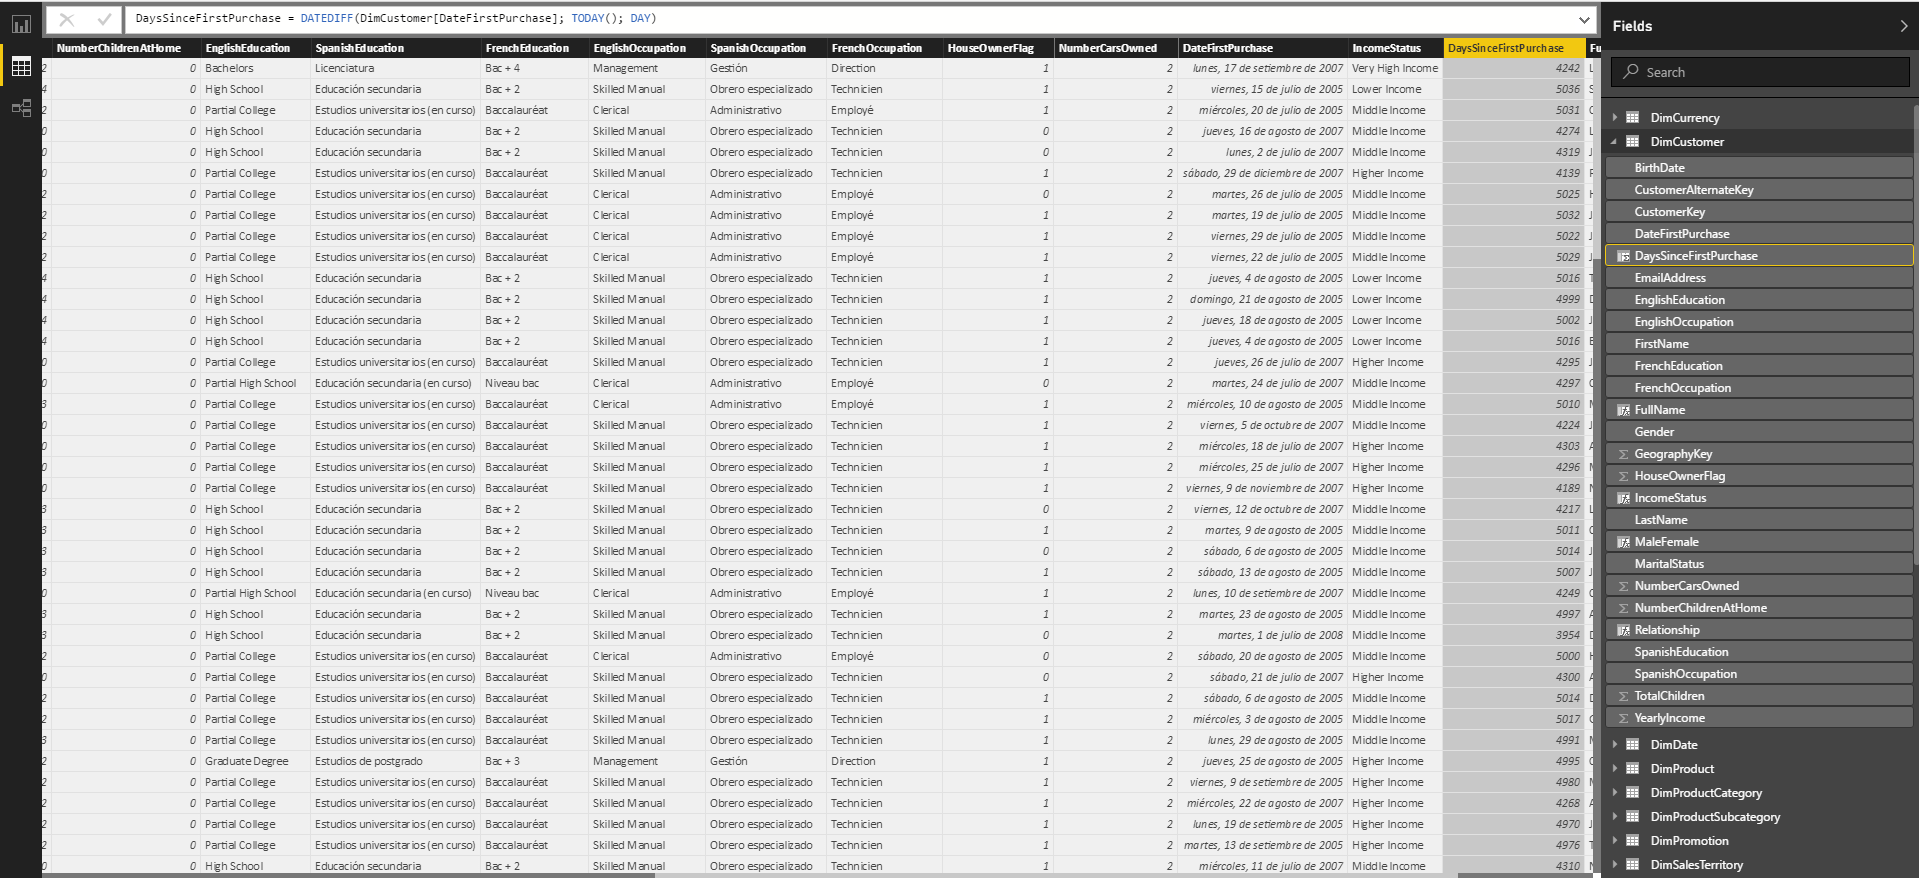
\includegraphics[width=17cm]{./Imagenes/32} 
	\end{center}


	\item En Power BI Desktop, haga clic en Datos en el panel de vistas en el lado izquierdo. En el panel Campos, haga clic en DimCustomer.  En la cinta Modelado, en el grupo Cálculos, haga clic en Nueva columna. En la barra de fórmulas, resalte Columna = y escriba:
	\\
	
			 
	\begin{center}
	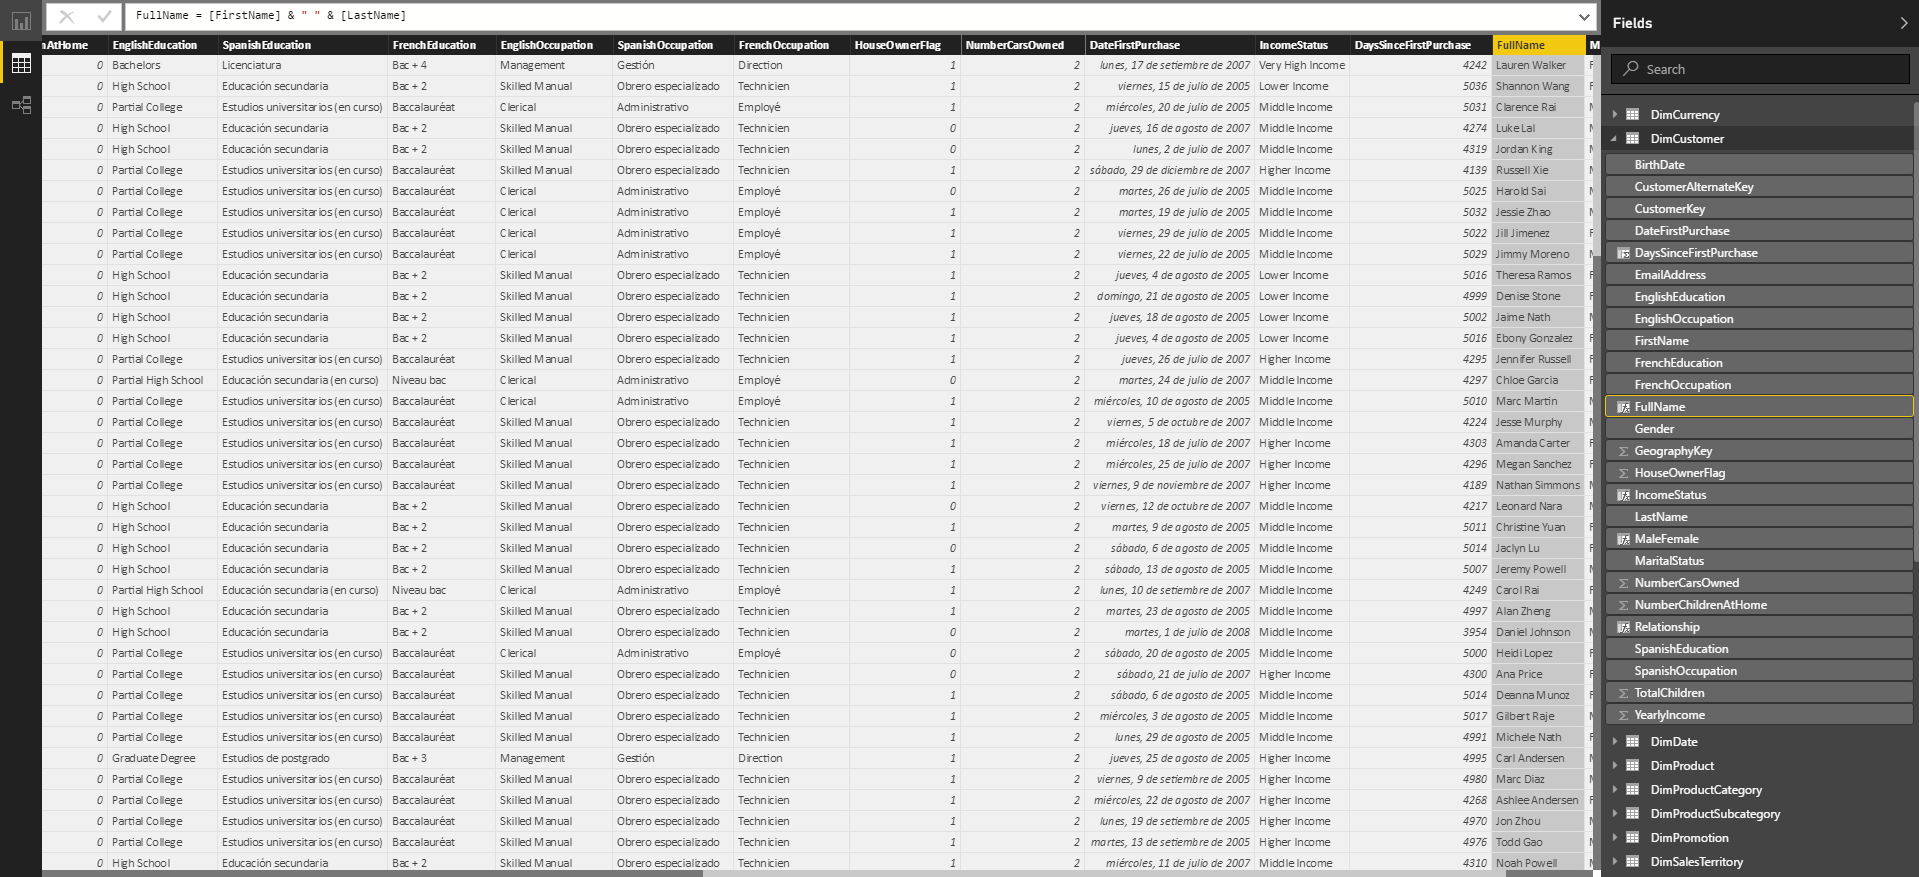
\includegraphics[width=17cm]{./Imagenes/33} 
	\end{center}


	\item En Power BI Desktop, haga clic en Datos en el panel de vistas en el lado izquierdo. En el panel Campos, haga clic en DimCustomer.  En la cinta Modelado, en el grupo Cálculos, haga clic en Nueva columna. En la barra de fórmulas, resalte Columna = y escriba:
	\\
	\\MaleFemale = IF([Gender] = "M", "Male", "Female")\\
			 
	\begin{center}
	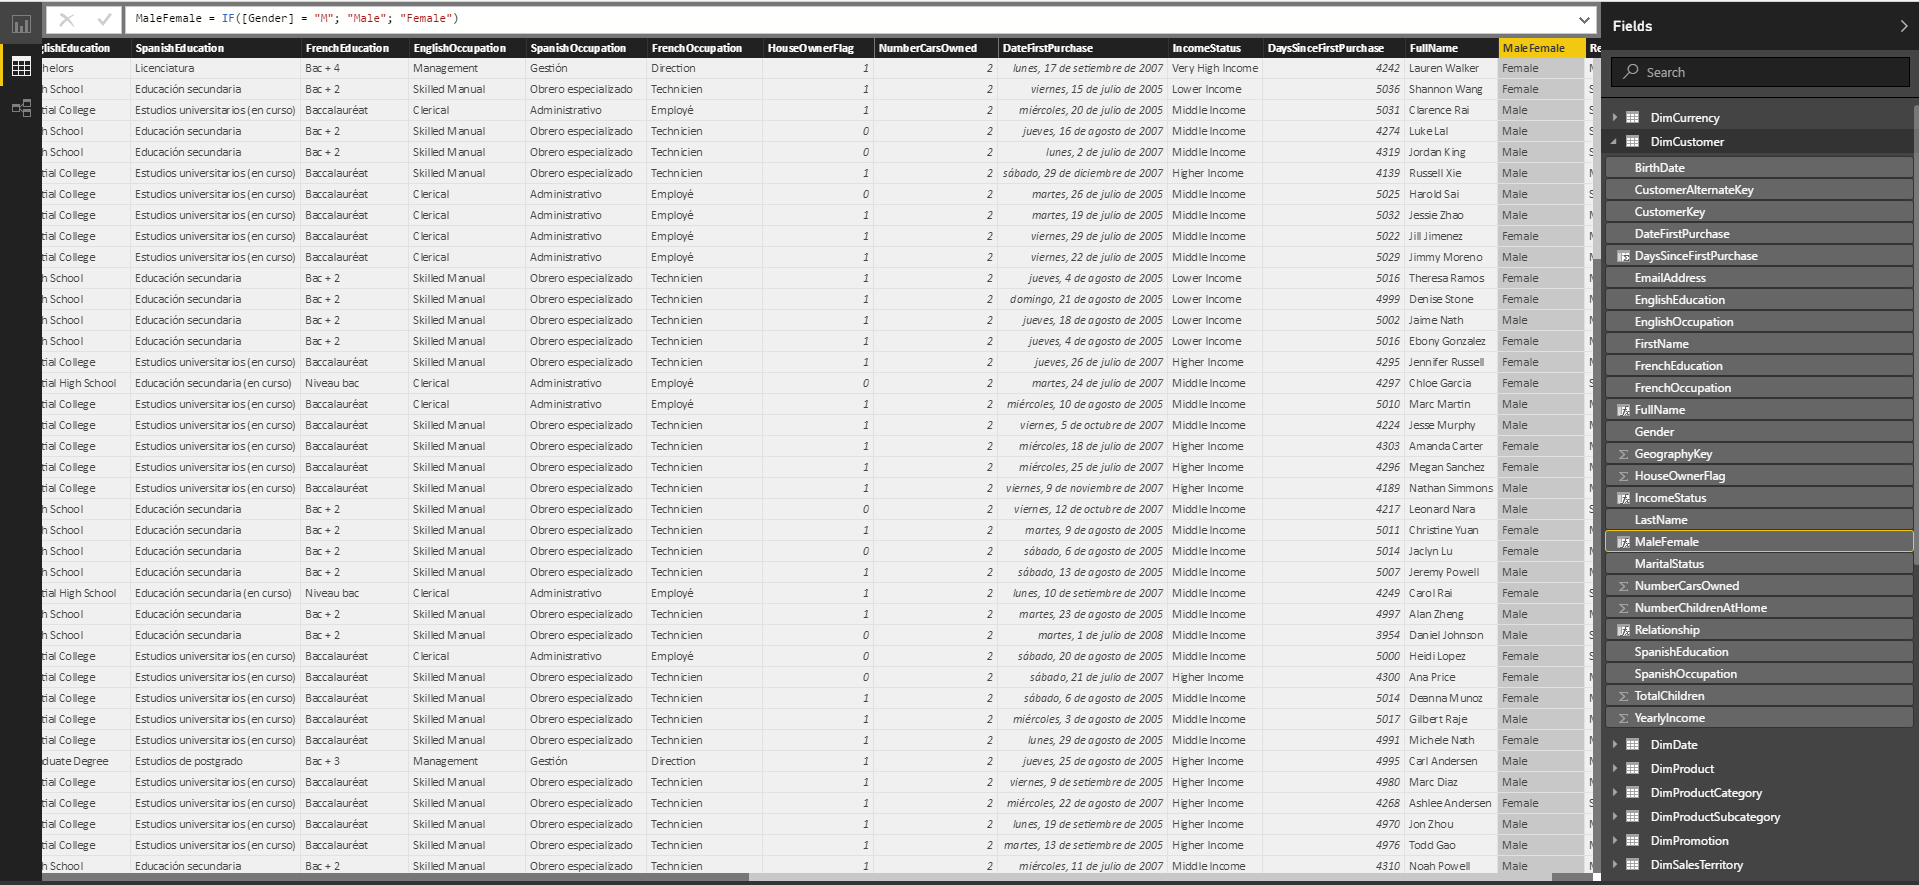
\includegraphics[width=17cm]{./Imagenes/34} 
	\end{center}

	\item En Power BI Desktop, haga clic en Datos en el panel de vistas en el lado izquierdo. En el panel Campos, haga clic en DimCustomer.  En la cinta Modelado, en el grupo Cálculos, haga clic en Nueva columna. En la barra de fórmulas, resalte Columna = y escriba:
	\\
	\\Relationship = IF([MaritalStatus] = "M", "Married", "Single")\\
			 
	\begin{center}
	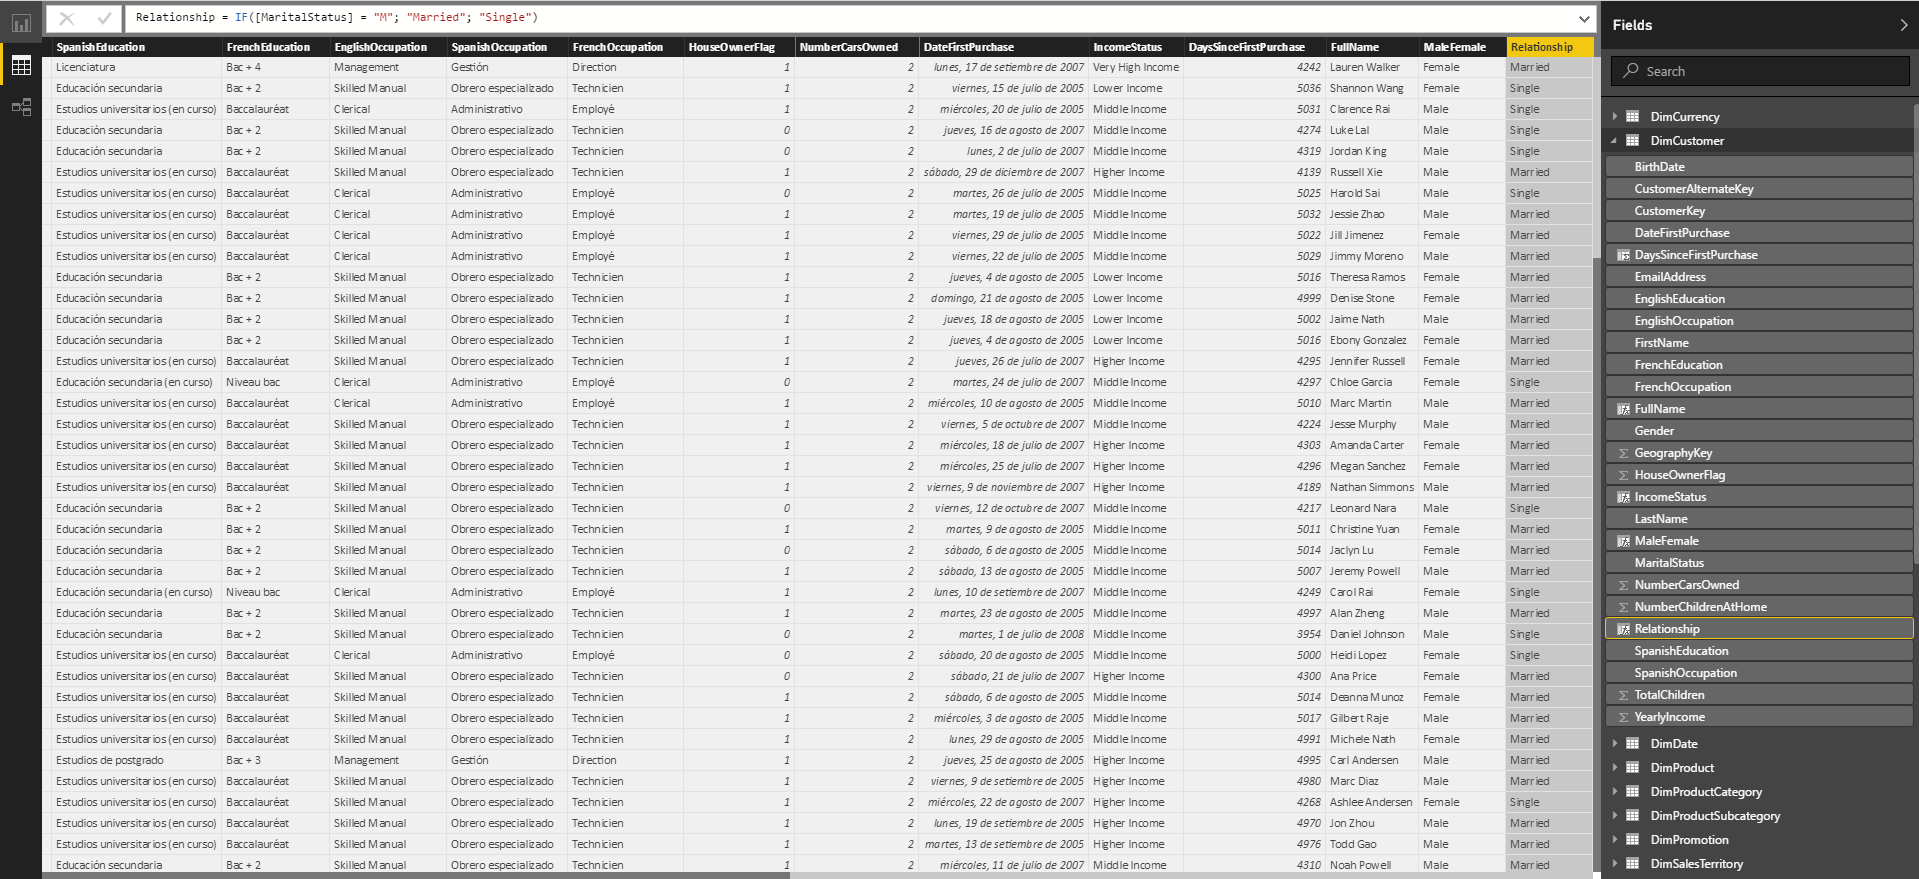
\includegraphics[width=17cm]{./Imagenes/35} 
	\end{center}

	\item En Power BI Desktop, haga clic en Datos en el panel de vistas en el lado izquierdo. En el panel Campos, haga clic en DimCustomer.  En la cinta Modelado, en el grupo Cálculos, haga clic en Nueva columna. En la barra de fórmulas, resalte Columna = y escriba:
	\\
	\\MainCategory = RELATED(DimProductCategory[CategoryName])\\
			 
	\begin{center}
	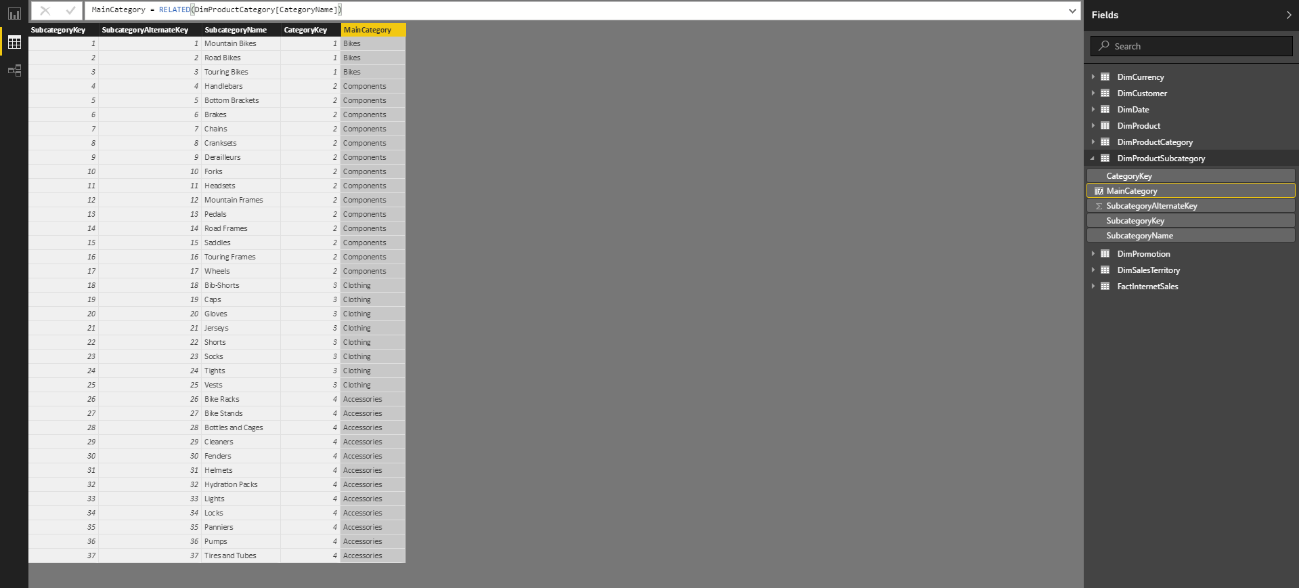
\includegraphics[width=17cm]{./Imagenes/36} 
	\end{center}

	\item En Power BI Desktop, haga clic en Datos en el panel de vistas en el lado izquierdo. En el panel Campos, haga clic en DimPromotion.  En la cinta Modelado, en el grupo Cálculos, haga clic en Nueva columna. En la barra de fórmulas, resalte Columna = y escriba:
	\\
	\\PromotionLengthDays = DATEDIFF(DimPromotion[StartDate], DimPromotion[EndDate], DAY)\\
			 
	\begin{center}
	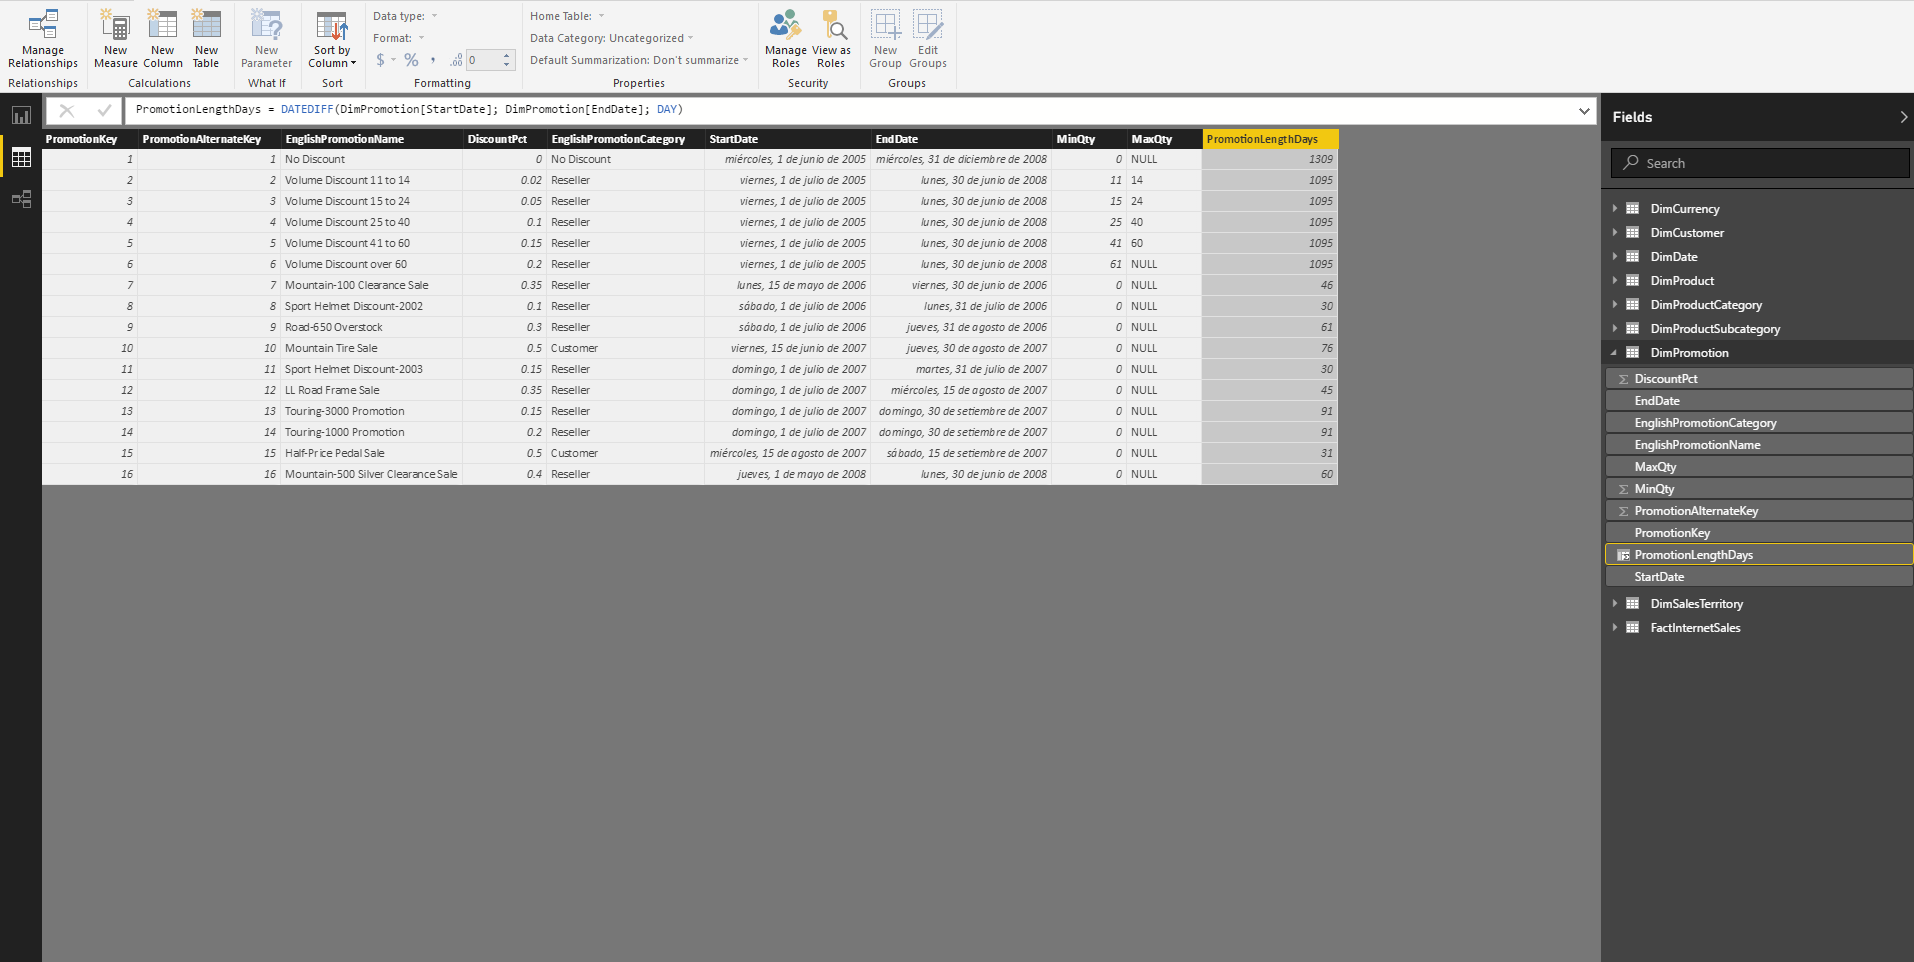
\includegraphics[width=17cm]{./Imagenes/37} 
	\end{center}


	\item En Power BI Desktop, haga clic en Datos en el panel de vistas en el lado izquierdo. En el panel Campos, haga clic en DimPromotion.  En la cinta Modelado, en el grupo Cálculos, haga clic en Nueva columna. En la barra de fórmulas, resalte Columna = y escriba:
	\\
	\\Profit = CURRENCY(FactInternetSales[UnitPrice] - \\
FactInternetSales[ProductStandardCost])\\
			 
	\begin{center}
	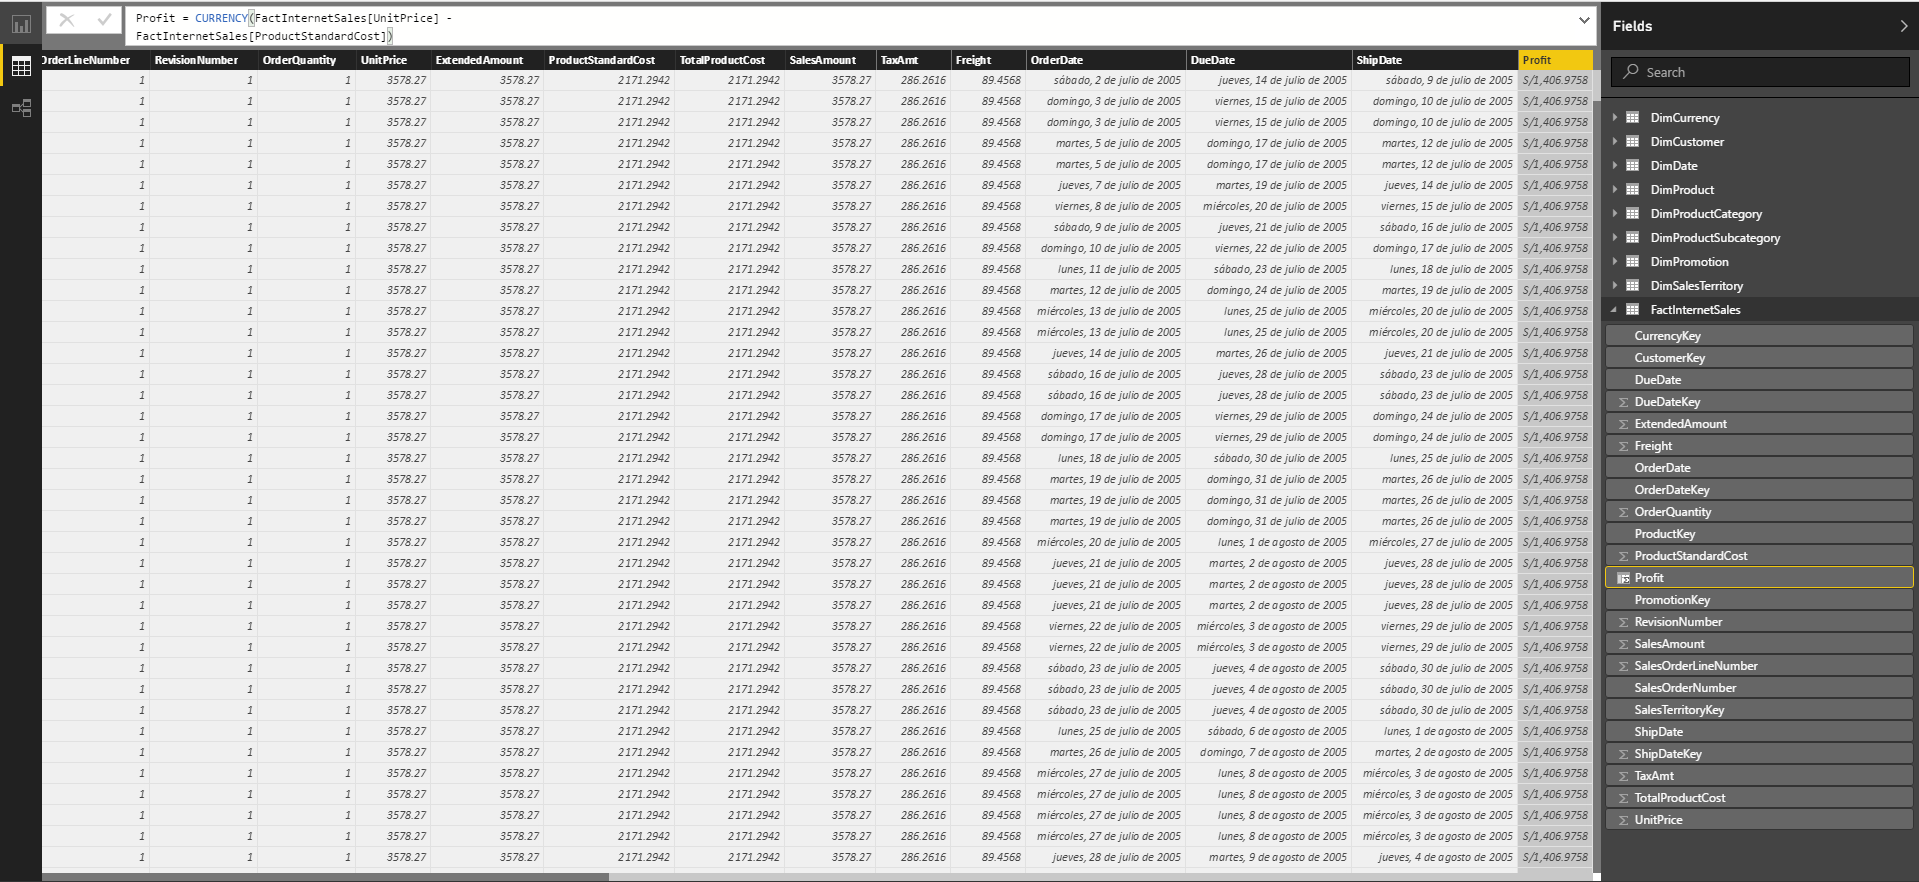
\includegraphics[width=17cm]{./Imagenes/38} 
	\end{center}

\end{enumerate}







\end{document}
